\documentclass{article}
\usepackage{MAECapstoneCourse,amsmath,graphicx,url,times}
\usepackage{color}
\usepackage[utf8]{inputenc}
\pagenumbering{arabic}

\newcommand{\quotes}[1]{``#1''}

\title{Real-time neural audio effects processing based on parametric training}

% PUT NAMES IN ALPHABETIC ORDER (consider surname first)
\name{Edoardo Morena, Niccolò Perego}
\address{Dipartimento di Elettronica, Informazione e Bioingegneria (DEIB), Politecnico di Milano\\
Piazza Leonardo Da Vinci 32, 20122 Milano, Italy\\   
\tt{[edoardo.morena,niccolo.perego]@mail.polimi.it}    
}

\begin{document}

\ninept
\maketitle

\begin{sloppy}

\begin{abstract}
This paper presents a plugin that highlights the potential of neural network-based computing as a new frontier in the audio processing field. The presented plugin showcases the  capabilities of neural networks dwelling on the parametric training method, offering a glimpse into the future of sound design and production. As neural network technologies continue to evolve, the possibilities for pushing the boundaries of audio manipulation are both exciting and vast.
\end{abstract}

\begin{keywords}
Audio, Neural Networks, Plugin, Audio Effect
\end{keywords}

\section{Introduction}
\label{sec:intro}

Over the past few years, the integration of neural networks into audio processing systems has emerged, revolutionizing the landscape of sound manipulation. This paper presents a novel audio plugin that exploits the power of parametric neural network training to achieve two distinct real-time audio effects: distortion and low pass filtering. Thanks to the versatility of neural networks, the proposed plugin offers impressive control and customization for sound engineers and music producers.


The plugin leverages the \emph{PyTorch} library for model definition and training, employing Long Short-Term Memory (LSTM) architectures to capture the intricate nuances of audio signals. Notably, a single audio file serves as the foundation for generating diverse datasets essential for training.

In this paper, we also aim at illustrating, through visual representations, the impact of utilizing LSTM models of varying dimensions, highlighting the differences in performance and capabilities across different architectural choices.

Moreover, the plugin effectively demonstrates the power of neural training by providing users with the unique capability to exploit its functionalities for mapping plugin controls. This type of feature, that we called \quotes{SuperKnob}, showcases the potential for dynamic and personalized audio manipulation.

\section{TRAINING}
\label{sec:training}

\subsection{Dataset}
\label{ssec:dataset}
The dataset is generated from one (or more) input audio file, partitioned into smaller fragments. With this approach we are able to represent various audio characteristics within a unified dataset. Each audio fragment is paired with a corresponding parameter value, yielding a dual-channel structure in the form of a NumPy array. One channel contains the audio fragment, while the other channel features a repeated instance of the associated parameter value, establishing a two-dimensional representation.

This dual-channel structure forms the input to our neural network models, effectively integrating conditional informations into the training process. Each input fragment is correlated with an output segment, an audio counterpart of the input fragment. However, the output segment presents a certain degree of audio effect (either distortion or low pass filtering), with an intensity determined by the accompanying parameter.

The coupling of input fragments with a conditional value enhances the network's capacity to learn the intricate relationship between audio content and effect parameters. In the subsequent sections, we delve into the architecture and training specifics of the neural networks used in the plugin, shedding light on the dynamic process that empowers the its processing capabilities.

\subsection{Model Selection}
\label{ssec:modelSel}

We conducted multiple tests to determine the neural architecture that best suited our objectives. Leveraging the \emph{PyTorch} library, we explored several models, with an emphasis on attaining optimal real-time inference performance. 

To facilitate the integration into the plugin structure, we relied on a specialized tool named \emph{RTNeural}. This library, thanks to its ability to define a model architecture at compile time, excels in ensuring optimal inference speed, an important attribute for achieving real-time audio processing.

Our architecture choices, however, were limited by the constraints imposed by \emph{RTNeural}, which offers the possibility to adopt only a selection of specific neural network layers. Notably, our exploration comprised two primary architectures: Long Short-Term Memory (LSTM) networks and Convolutional Neural Networks (Conv1D).

The LSTM architecture's ability to process sequential data aligns perfectly with the audio signals' temporal nature. This made it a perfect candidate for our investigation. Additionally, we explored the abilities of Conv1D networks, which specialize in capturing local patterns within sequential data. We observed that LSTM architectures yielded superior results compared to Conv1D networks, both in terms of validation loss values and in preserving the timbral characteristics of the audio effect.

Thus, we proceeded comparing various LSTM models with different number and size of hidden layer. To evaluate the impact of size on model performance, we contrasted the outcomes of an LSTM model with 16 hidden cells against that of a model with 32 hidden cells. What we noted is that the first, \quotes{LSTM16}, exhibited comparable results with respect to second, \quotes{LSTM32}, across various audio manipulation tasks. Given this parity in outcomes we realized that a smaller, less complex model would better ensure optimal real-time performance. We then opted for the 16-hidden layer architecture. 

Graphical representations illustrating the comparison between these architectures are presented in the dedicated results section. These insights are useful to understand the importance of neural network selection but also to highlight the crucial role of model size in attaining optimal performance within the real-time audio processing task.

\subsection{Parametric Training}
\label{ssec:parTraining}
The conditional training of the models was successfully accomplished utilizing the computational power of GPUs provided by Google Colab and exploiting the capabilities of the \emph{PyTorch} library. Each input audio segment, along with its corresponding parameter, was paired with an output segment featuring an effect intensity depending on the parameter value. This output segment served as the target for the model, enabling it to learn the intricate relationships between input, parameter, and output. The training process was facilitated through the \emph{Adam} optimizer, a widely-used optimization algorithm that adapts learning rates, enhancing convergence speed and accuracy.

Regarding the loss function, it's worth mentioning the adoption of a \texttt{LossWrapper}. This class efficiently computes a consolidated loss by considering the model's output and the corresponding target signal. This unified loss combines various loss functions, notably the \emph{Error to Signal} Loss and the \emph{DC} Loss. This approach significantly contributed to refining the neural network models, yielding improved audio transformations.

To further speed up the process, the entire dataset was divided into manageable batches, allowing efficient computations and model updates. This approach enabled the networks to effectively learn the intricacies of audio transformation, culminating in the plugin's ability to dynamically adjust its effects in response to user-controlled parameters.

Once the training is completed the model is saved and exported as a \texttt{json} file, making the import in the plugin with \emph{RTNeural} feasible.


\section{PLUGIN IMPLEMENTATION}
\label{sec:pluginInterpretation}
The audio plugin was implemented in \texttt{C++}, leveraging the capabilities of the \emph{JUCE} library. This choice facilitated the creation of a versatile and efficient platform for audio processing, hosting both the audio and the graphical user interface (GUI) components of the plugin. To ensure optimal real-time performance, the \emph{RTNeural} library was incorporated, allowing to import the trained neural models.

Furthermore, the integration of the \emph{libtorch} added offered an unique layer to the plugin's functionalities. Through this, the concept of a \quotes{SuperKnob} was developed.

Fundamental to the user experience is the plugin's GUI, which offers diverse possibilities for user interaction with the neural models, guaranteeing an intuitive and immersive experience. In this paper, we will explain the details of the GUI design and its integration with the underlying neural networks.


\subsection{Inference}
\label{ssec:inference}
The inference process is probably the most important step in the plugin's audio processing pipeline. As the incoming audio signal enters the plugin, it serves as the primary input for the model imported using \emph{RTNeural}. Simultaneously, the parameter values extracted from the GUI controls add a critical conditional aspect, controlling the audio transformation. For each of the effects, the neural model processes this combination of input and parameter, generating an output that embodies the desired effect.

The output from the neural model is then audibly presented to the user, creating a dynamic and real-time audio experience. The input signal traverses two distinct neural networks, beginning with the distortion model before proceeding through the LPF model. This dual-stage transformation accentuates the plugin's versatility, enabling users to seamlessly combine the effects as desired.

A noteworthy feature is the possibility for users to select from a range of pre-trained neural models, each embodying a unique conditional training approach. This diversity empowers the users to explore and personalize the audio transformation process based on their creative intentions.

Importantly, the integration of \emph{RTNeural} speeds up the inference process by compiling the neural network architecture only once, at compile time. This architectural definition approach significantly accelerates inference times, enabling the plugin to operate with remarkable speed and responsiveness. We wanted the plugin to offer users an immersive and dynamic audio manipulation experience.

While the incorporation of \emph{RTNeural} and its optimizations significantly enhances real-time responsiveness, it is noteworthy that utilizing an excessively large hidden layer size in the LSTM architecture can still pose challenges to achieving smooth real-time performance, potentially compromising the user experience.

\subsection{GUI and Functionalities}
\label{ssec:gui}

\begin{figure}[t]
  \centering
  \centerline{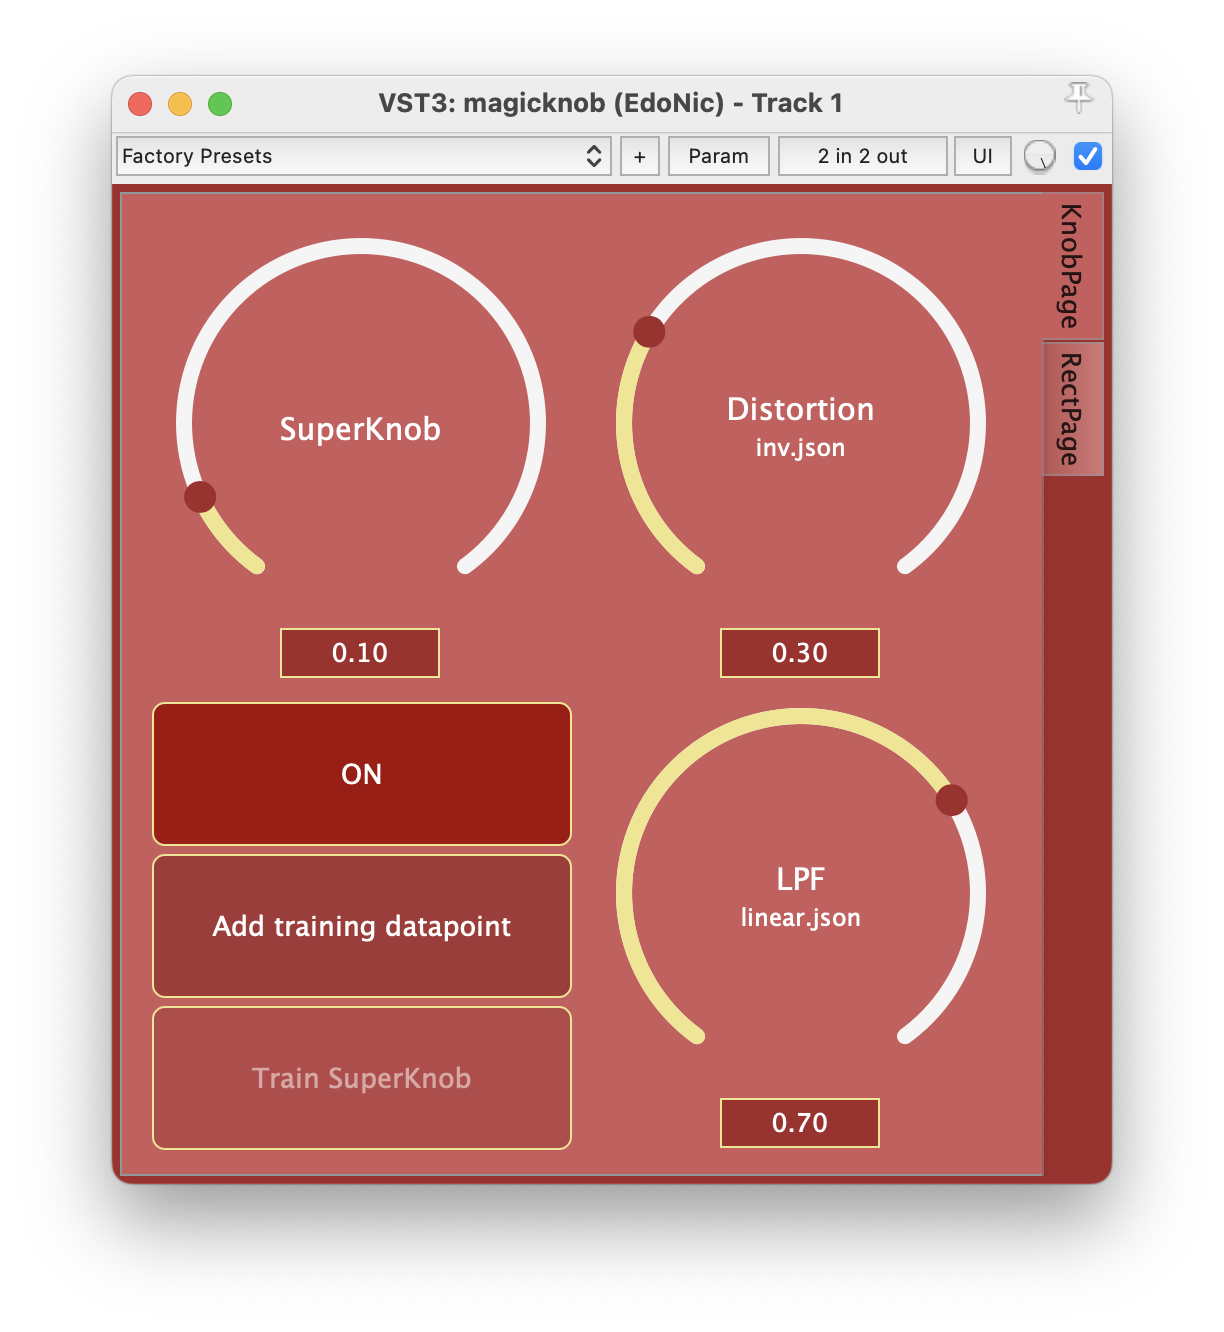
\includegraphics[width=\columnwidth]{images/knobPage.png}}
  \caption{GUI - KnobPage}
  \label{fig:knobPage}
\end{figure}

\begin{figure}[t]
  \centering
  \centerline{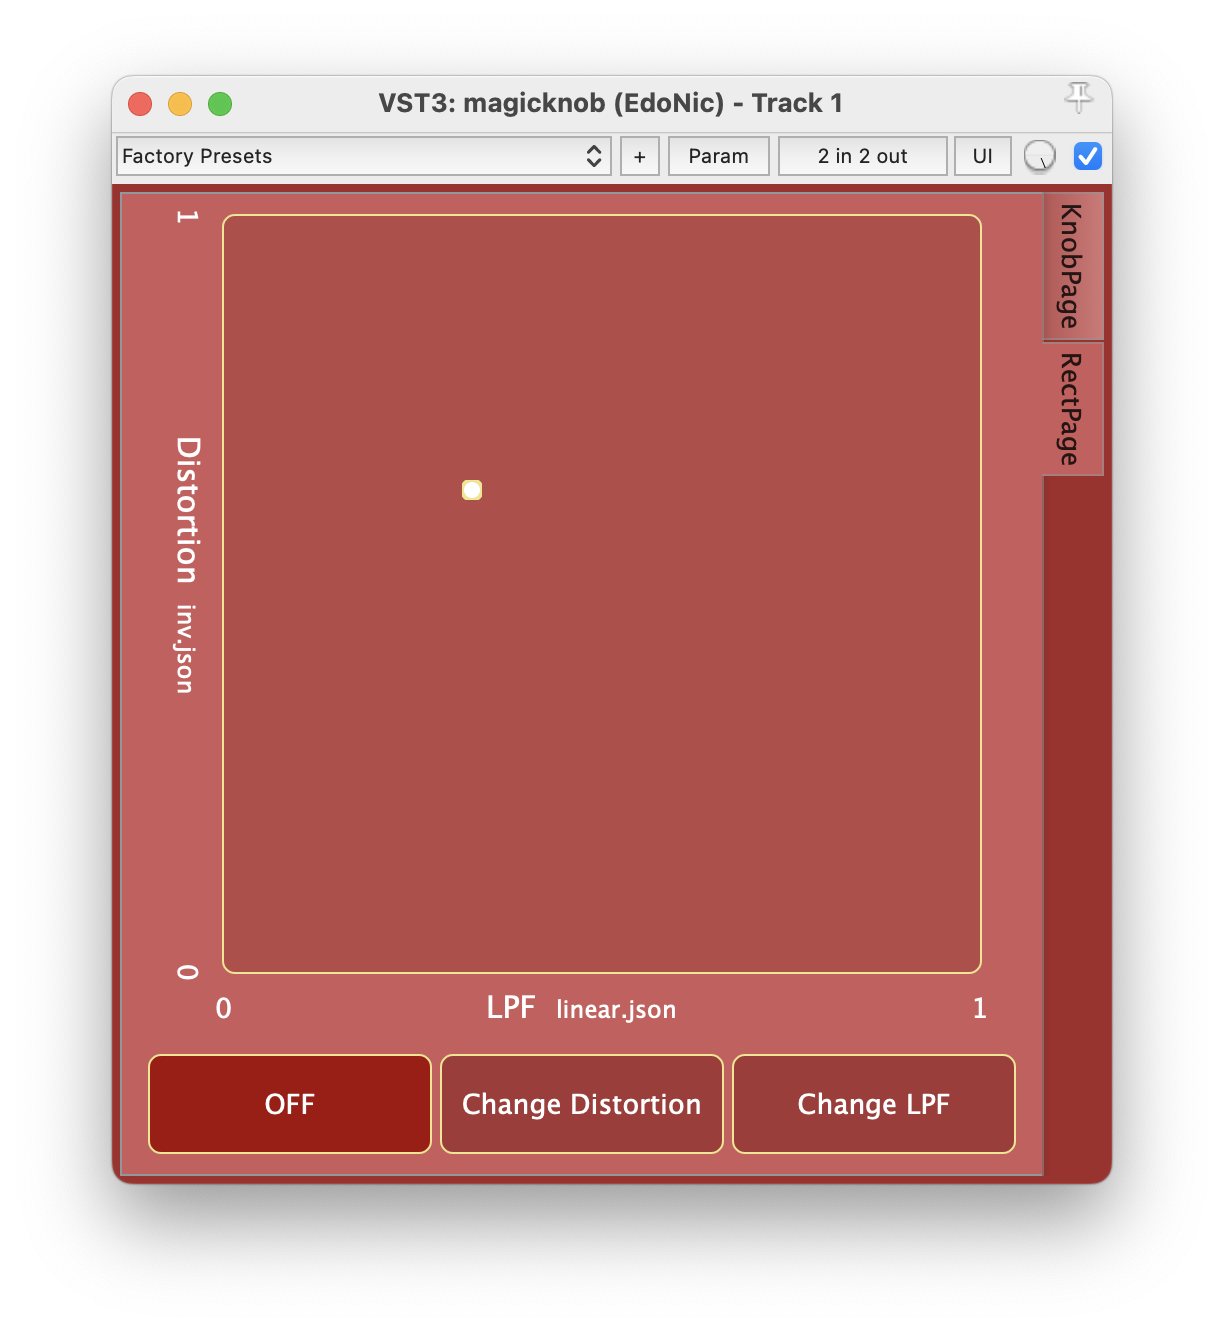
\includegraphics[width=\columnwidth]{images/rectPage.png}}
  \caption{GUI - RectPage}
  \label{fig:rectPage}
\end{figure}

The graphical user interface (GUI) of the plugin is basically divided into two distinct screens, each offering users diverse modes of interaction with the neural effect. In Figure \ref{fig:knobPage} and \ref{fig:rectPage} we show how these two pages look. 

The initial screen, \texttt{KnobPage}, comprises dials for the distortion and the low pass filter effects, enabling their independent manipulation. Additionally, this screen houses all the essential controls necessary to implement the \quotes{SuperKnob} functionality. These include the primary control knob, a button for adding the current input value and the corresponding distortion and low pass filter knob values to the dataset, and a \quotes{Train} button to initiate training. Once a model is ready, this last button offers the possibility to reset the training process and create a new \quotes{SuperKnob} setting from scratch. This particular functionality enables users to operate both effect knobs by simply adjusting the \quotes{SuperKnob} and to explore the value space by means of neural training.

The second tab, \texttt{RectPage}, provides the users with a Cartesian space for parameter exploration. Here, users can navigate the entire parameter values space using a cursor positioned within the plane. The y-axis corresponds to the distortion amount, while the x-axis governs the opening or closing of the low pass filter. Two buttons offer to the users the ability to swiftly switch between different pre-trained neural models for both distortion and low pass filtering effects, enhancing the plugin's adaptability. In the first page the user can switch between these models by double-clicking the single effect knobs.

Incorporating these functionalities into the plugin's GUI enhances user engagement, facilitating intuitive and dynamic control over the audio transformations. This interface empowers users to experiment with diverse combinations of effects, \quotes{SuperKnob} strategies, and model choices, letting them explore in a interactive fashion the realm of neural audio manipulation.

\section{RESULTS}
\label{sec:results}

\subsection{Model Evaluation}
\label{ssec:modelEval}

\begin{figure}[t]
  \centering
  \centerline{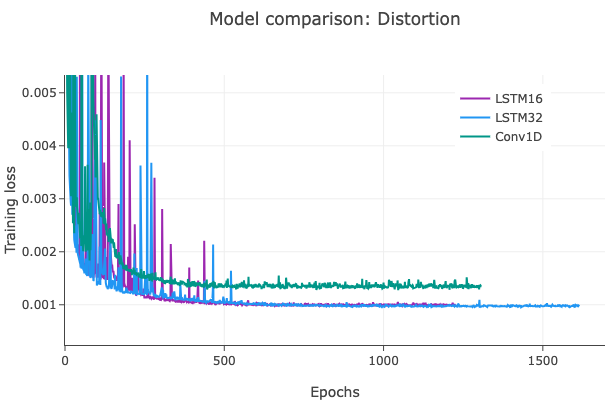
\includegraphics[width=\columnwidth]{./plots/trimmedImgs/dist trainLoss.png}}
  \caption{Distortion Effect - Training Loss Trajectories for Different Neural Architectures}
  \label{fig:distTrain}
\end{figure}

\begin{figure}[t]
  \centering
  \centerline{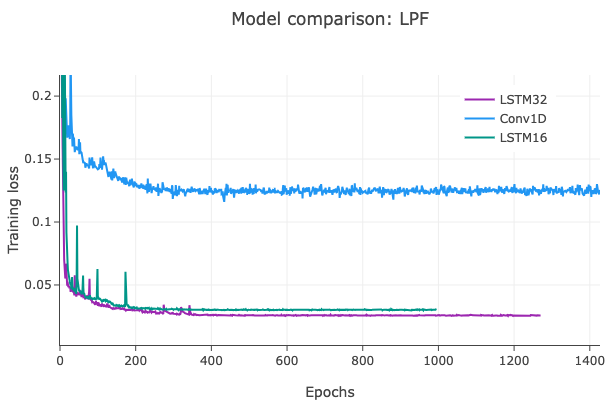
\includegraphics[width=\columnwidth]{./plots/trimmedImgs/lpf trainLoss.png}}
  \caption{LPF - Training Loss Trajectories for Different Neural Architectures}
  \label{fig:lpfTrain}
\end{figure}

\begin{figure}[t]
  \centering
  \centerline{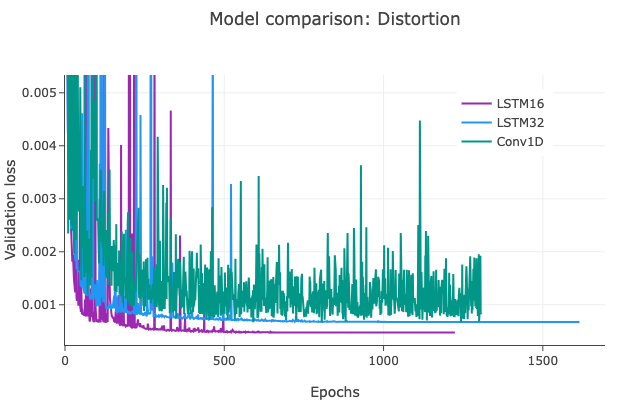
\includegraphics[width=\columnwidth]{./plots/trimmedImgs/dist valLoss.png}}
  \caption{Distortion Effect - Validation Loss Trajectories for Different Neural Architectures}
  \label{fig:distVal}
\end{figure}

\begin{figure}[t]
  \centering
  \centerline{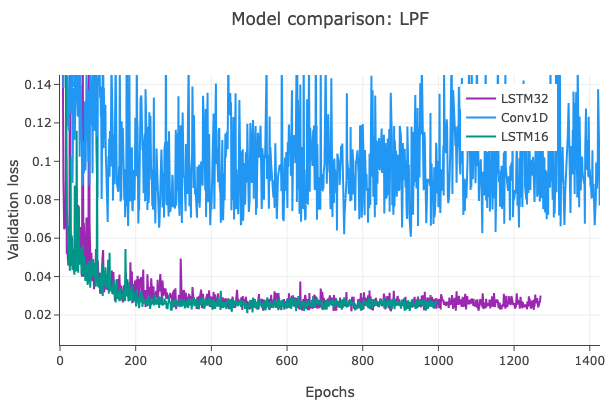
\includegraphics[width=\columnwidth]{./plots/trimmedImgs/lpf valLoss.png}}
  \caption{LPF - Validation Loss Trajectories for Different Neural Architectures}
  \label{fig:lpfVal}
\end{figure}

In this section, we provide a detailed visual representation of the achieved technical results, focusing on the impact of varying neural architectures within the context of a linear parameter conditioning. Each audio effect, distortion, and low pass filtering, is accompanied by a pair of graphs, one showcasing the training loss trajectories and another one regarding the validation loss. Within each pair, we unveil the dynamics of the losses  throughout the training epochs.

The presented loss curves reflect the influence of the \quotes{linear} parameter conditioning strategy. This methodology dictates that as the parameter value increases, both the distortion intensity and the opening of the low pass filter should proportionally escalate. Such an approach enhances the intuitive control and manipulation of the audio effects.

Our analysis comprehends three distinct neural network architectures: an LSTM-based model with a hidden layer dimension of 16, an LSTM-based model with a hidden layer dimension of 32, and a Conv1D-based model. This last model mimics an encoder-decoder structure, even though we couldn't resort to \emph{Transposed Convolution} layers due to their unavailability in \emph{RTNeural}. Through these graphical representations, we show the loss trajectories of these architectures and provide a comparative overview of their ability to capture the intricacies of linear parameter-based audio transformation.

The Conv1D-based architecture shows relatively inferior performance compared to the others, as evidenced by both training and validation results in Figure \ref{fig:distTrain}, \ref{fig:lpfTrain}, \ref{fig:distVal} and \ref{fig:lpfVal}. Particularly noteworthy is its struggle to model the Low Pass Filter (LPF) effect, as indicated by the incapability to achieve an accurate audio response. These limitations are evident throughout the training and validation loss trends, emphasizing the Conv1D's relative inefficacy in capturing the characteristics of the LPF effect. In contrast, both the \quotes{LSTM16} and \quotes{LSTM32} models demonstrate great performances, with both architectures showcasing proficient results. However, the \quotes{LSTM16} model displays a slightly superior outcome in terms of validation loss, particularly when considering the distortion effect, as shown in Figure \ref{fig:distVal}.

\subsection{Model Selection}
\label{ssec:modelSelRes}

\begin{figure}[t]
  \centering
  \centerline{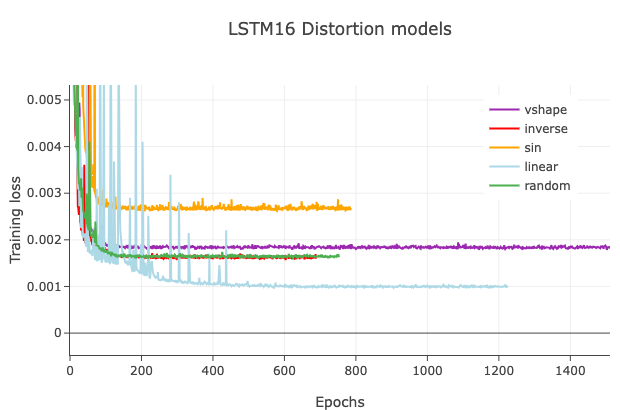
\includegraphics[width=\columnwidth]{./plots/trimmedImgs/dists trainLoss.png}}
  \caption{Distortion Effect - Training Loss Trajectories for Different Conditioning Strategies}
  \label{fig:distsTrain}
\end{figure}

\begin{figure}[t]
  \centering
  \centerline{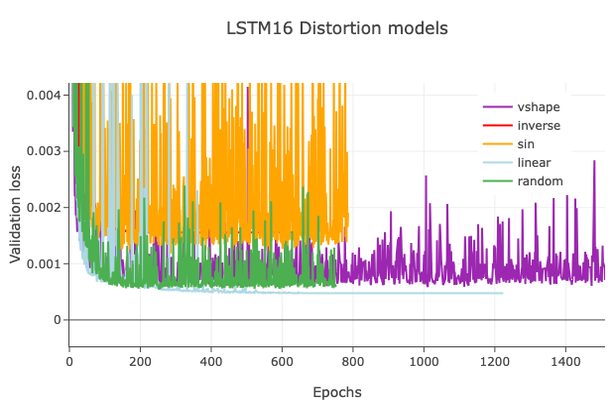
\includegraphics[width=\columnwidth]{./plots/trimmedImgs/dists valLoss.png}}
  \caption{Distortion Effect - Validation Loss Trajectories for Different Conditioning Strategies}
  \label{fig:distsVal}
\end{figure}

\begin{figure}[t]
  \centering
  \centerline{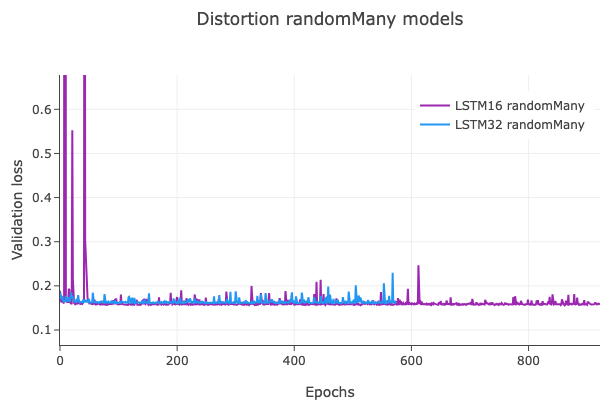
\includegraphics[width=\columnwidth]{./plots/trimmedImgs/randomMany dist trainLoss.png}}
  \caption{Distortion Effect - Training Loss Trajectories for the \quotes{Random Many} Conditioning}
  \label{fig:randomManyTrain}
\end{figure}

\begin{figure}[t]
  \centering
  \centerline{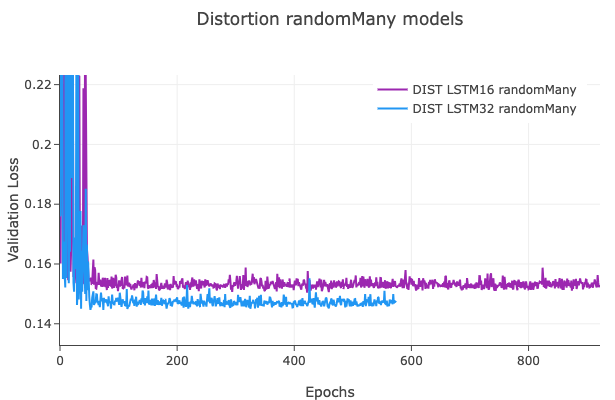
\includegraphics[width=\columnwidth]{./plots/trimmedImgs/randomMany dist valLoss.png}}
  \caption{Distortion Effect - Validation Loss Trajectories for the \quotes{Random Many} Conditioning}
  \label{fig:randomManyVal}
\end{figure}

Upon analysis of the graphs and informed by empirical assessments achieved through auditory evaluations of the embedded models, we arrived at the discerning decision to adopt the \quotes{LSTM16} architecture as the optimal choice for the plugin's operation. This architecture exhibited great performance and accurate audio transformations. Furthermore, having less parameters assures better real-time capabilities.

To provide further insights into our selection process, we present two additional graphs showcasing the training and validation loss trends for the distortion effect (Figure \ref{fig:distsTrain} and \ref{fig:distsVal}). These graphs show the trajectories of different conditioning strategies, illustrating the models' adaptability and responsiveness to diverse parameter variations. 

Below is an itemized list detailing the employed conditioning strategies for the distortion effect, accompanied by concise descriptions:

\begin{itemize}
  \item \textbf{Linear}: As previously described, increasing the parameter value results in escalating distortion.
  \item \textbf{Inverse}: An increase in the parameter value corresponds to reduced distortion.
  \item \textbf{V-Shape}: Increasing the parameter initially reduces distortion, then amplifies it.
  \item \textbf{Sin}: The distortion intensity alternates between increasing and decreasing twice consecutively.
  \item \textbf{Random}: Five parameter values are used for conditional training, each associated with an output featuring a randomly assigned distortion value.
  \item \textbf{Random (Many)}: Similar to \quotes{Random}, but utilizing 50 parameter values instead of 5.
\end{itemize}

The graphs in Figure \ref{fig:distsTrain} and \ref{fig:distsVal} show the performance of the \quotes{LSTM16} architecture under a spectrum of parameter-based conditions, showcasing its capability to a diverse array of audio transformations.

The \quotes{LSTM16} architecture demonstrates robust performance on the linear and the inverse parameter conditioning strategy, displaying stable and favorable training and validation loss trends. In contrast, the other conditioning strategies yield higher variability and exhibit elevated minimum loss values. Despite this, the model consistently produces satisfactory audio effects across these varying strategies.

It's important to note that several experiments were conducted not necessarily to achieve precise loss trajectory patterns, but rather to push the model's limits and explore the potential for creating unconventional and intriguing audio effects. This experimental approach is particularly evident in strategies like \quotes{randomMany}, which is showcased in separeted graphs (Figure \ref{fig:randomManyTrain} and \ref{fig:randomManyVal}) due to its unique characteristics. As seen in this case of study, the minimum loss values are way higher then usual and it's worth noticing that a more complex architecture, like the \quotes{LSTM32}, actually showcases better results.

\subsection{Spectral Analysis and Information Enrichment}
\label{ssec:spectrAnalysis}

\begin{figure}[t]
  \centering
  \centerline{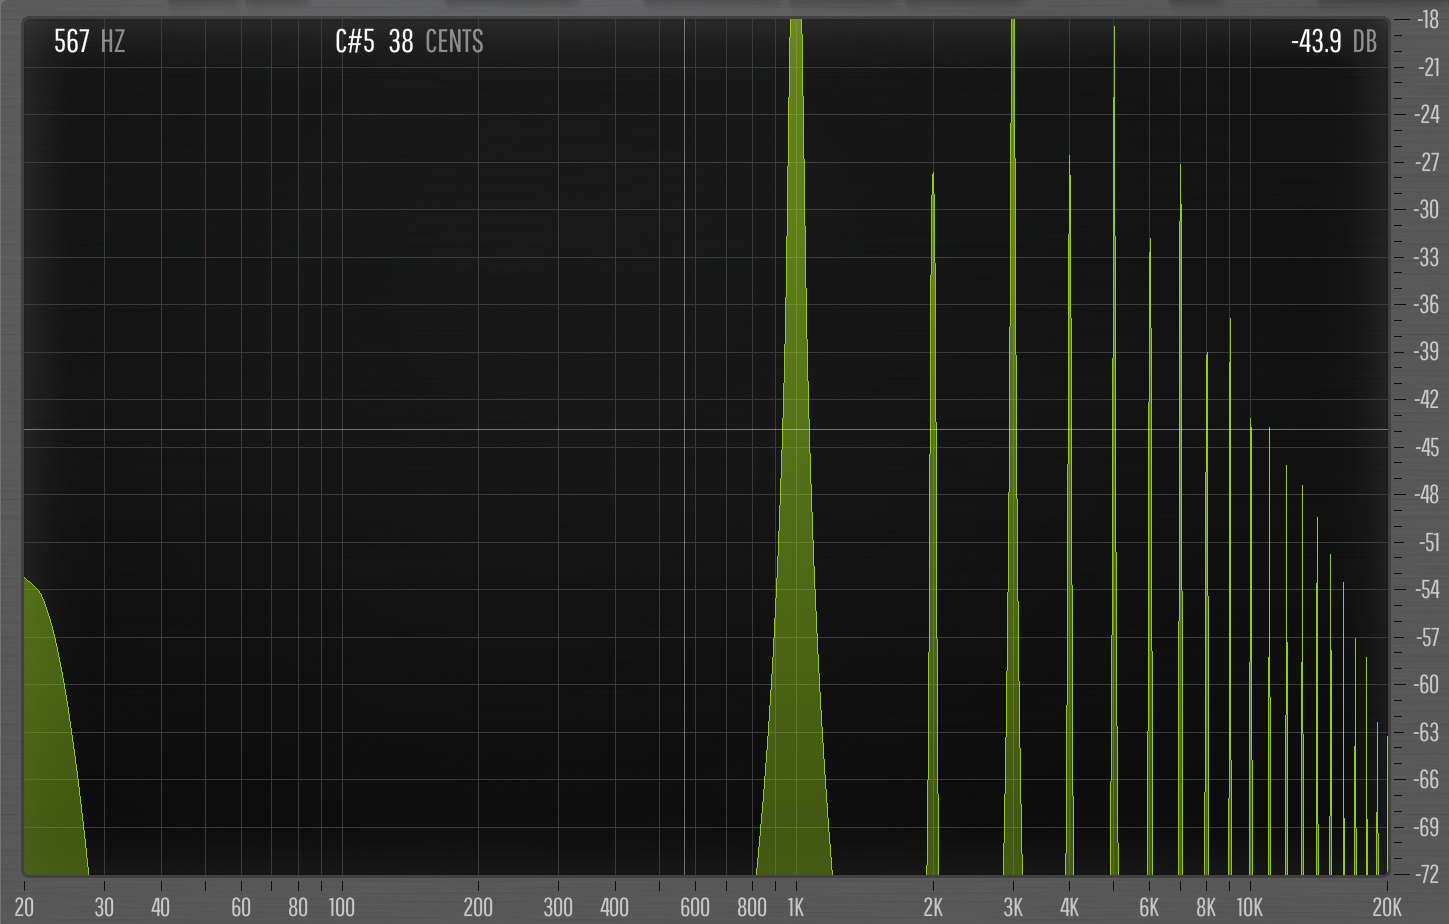
\includegraphics[width=0.95\columnwidth]{./images/dist vera.png}}
  \caption{Spectral Analysis - Logic Distortion Effect}
  \label{fig:logicDist}
\end{figure}

\begin{figure}[t]
  \centering
  \centerline{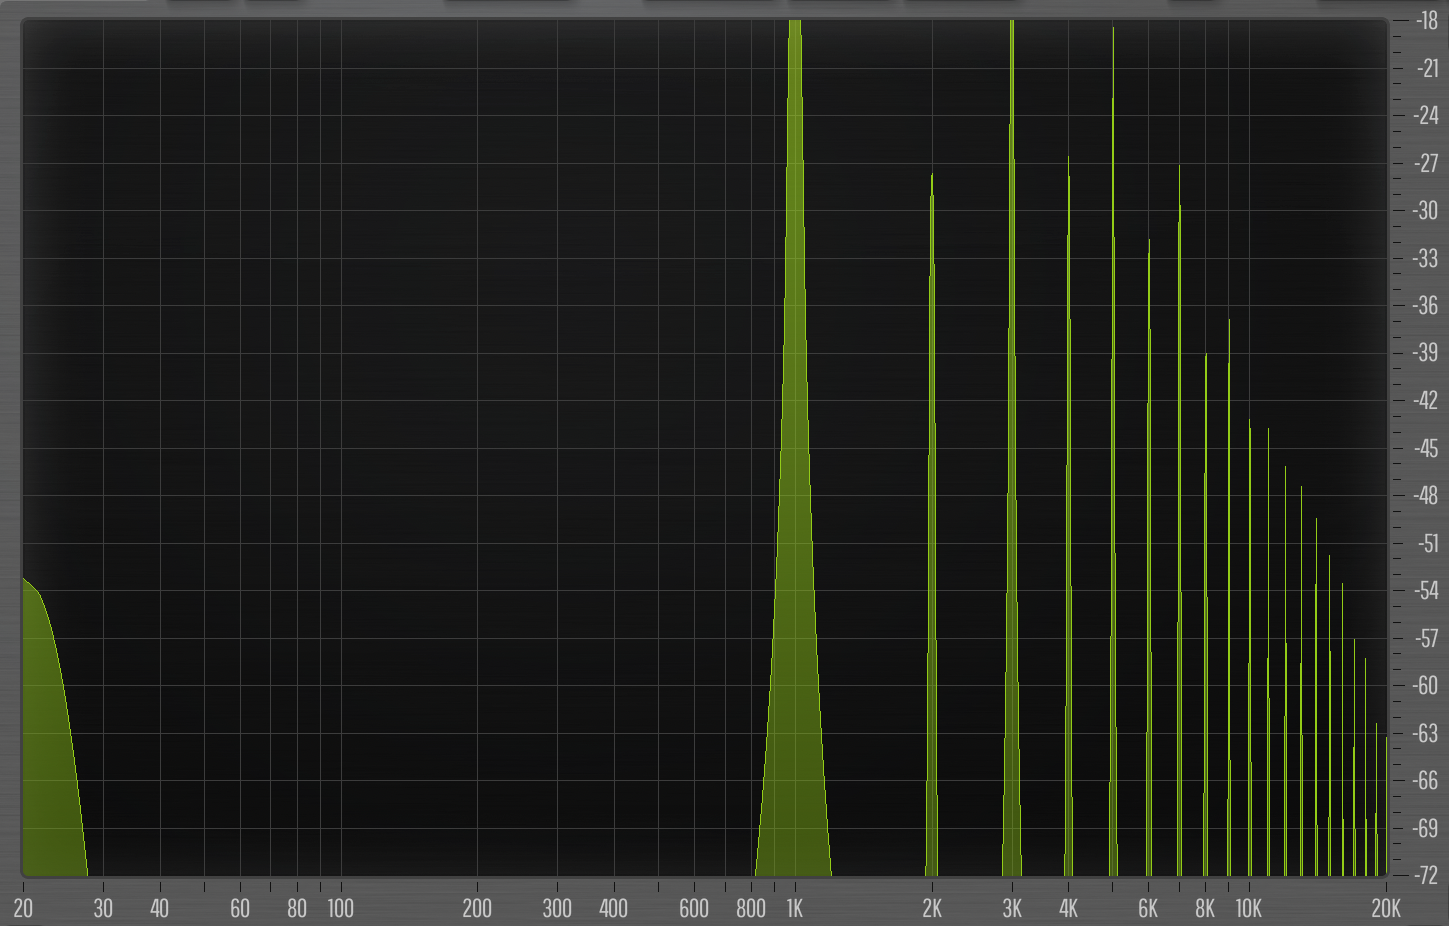
\includegraphics[width=0.95\columnwidth]{./images/dist magicknob.png}}
  \caption{Spectral Analysis - Neural-based Distortion Effect}
  \label{fig:ourDist}
\end{figure}

\begin{figure}[t]
  \centering
  \centerline{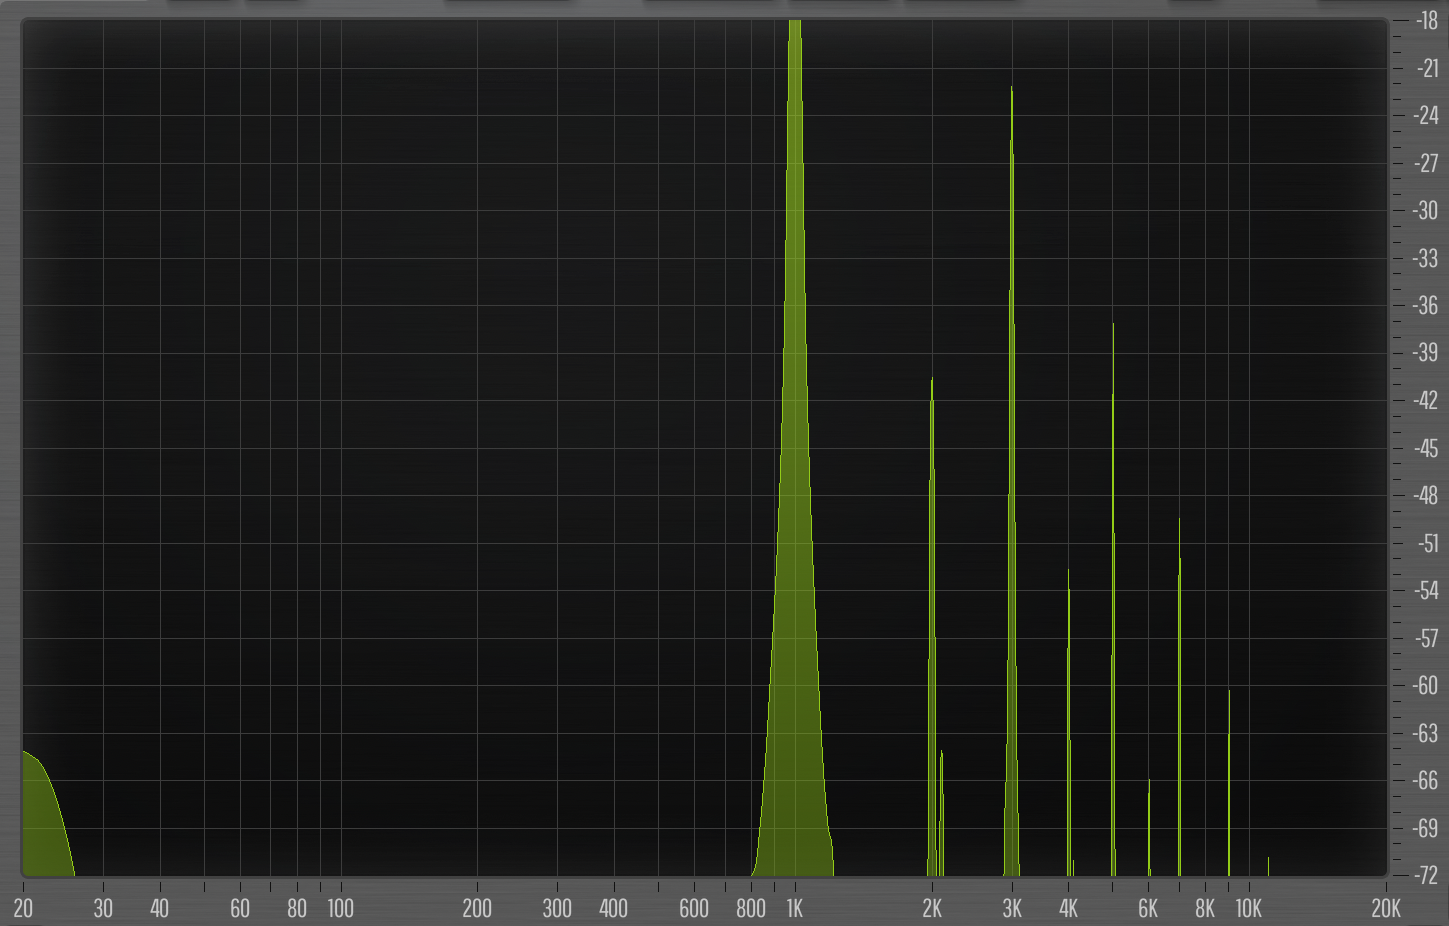
\includegraphics[width=0.95\columnwidth]{./images/dist lpf vera.png}}
  \caption{Spectral Analysis - Pro-Q 3 LPF Effect}
  \label{fig:proqLpf}
\end{figure}

\begin{figure}[t]
  \centering
  \centerline{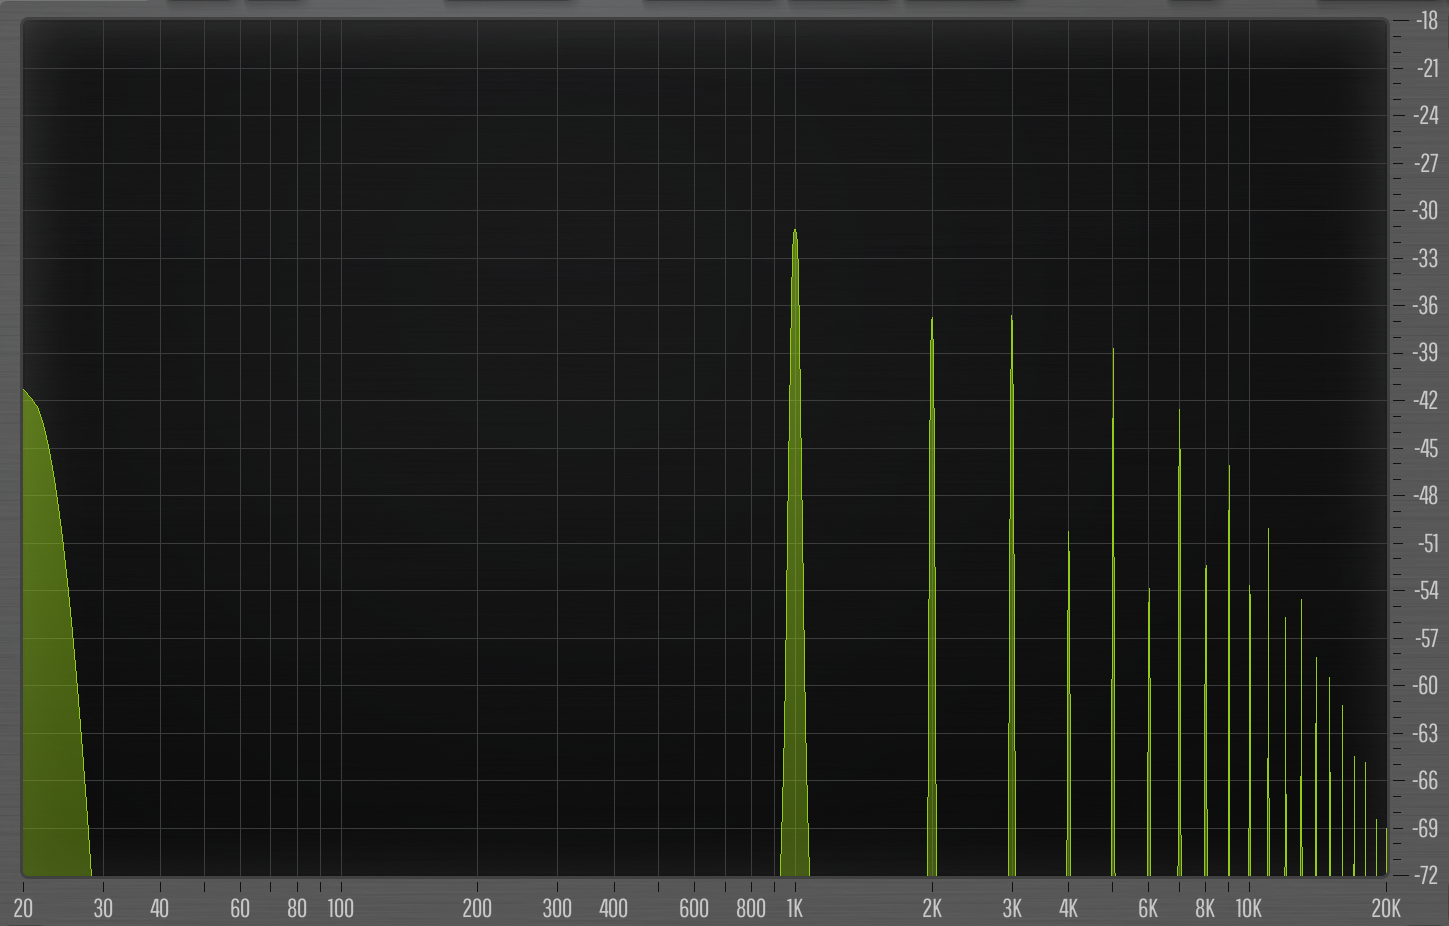
\includegraphics[width=0.95\columnwidth]{./images/dist lpf magicknob.png}}
  \caption{Spectral Analysis - Neural-based LPF Effect}
  \label{fig:ourLpf}
\end{figure}

In addition to evaluating the training performance through loss metrics, we conducted spectral analyses to visually depict how our plugin enhances frequency information compared to the standard effects it sought to model – a built-in distortion in Logic and low pass filter achieved with the FabFilter Pro-Q 3 equalizer. The
conducted spectral analyses uses a 1 kHz sinusoidal input signal.

The presented graphs (Figure \ref{fig:logicDist}, \ref{fig:ourDist}, \ref{fig:proqLpf} and \ref{fig:ourLpf}) showcase the spectral comparison between the the Logic distortion effect, the Pro-Q3 low pass filter effect (inserted after the distortion effect in order to show how it lowers the added harmonics), and the outcomes produced by our neural network-based plugin for both distortion and low pass filtering. These analyses reveal how our plugin enriches the frequency content of the input signal, offering more intricate and nuanced spectral transformations than their counterparts. The visual representation of the spectral analyses sheds light on the plugin's capacity to generate effects that retain the desired attributes of the target effects while introducing novel sonic characteristics through neural network-driven processing.

\section{CONCLUSIONS}
\label{sec:conclusions}

Finally, this project has delved into the application of neural networks in the audio processing field, resulting in the development of an audio plugin. Thanks to the \emph{PyTorch} library, together with \emph{RTNeural}, the plugin exploits neural networks to apply in real-time distortion and low pass filtering to audio signals. After several evaluations of different neural networks architectures we showed how \quotes{LSTM16} proved itself as the optimal choice, accurately capturing and modelling audio features.

We have showed different graphical proves demonstrating how the plugin can recreate different parameter conditioning strategies, letting the user explore in many ways the capabilities of neural modeling.

By combining neural networks with audio processing in a plugin that works in real time, we aimed at letting the users apply neural manipulation into their creative flux, exploring some of the possibilities that the neural network architectures offers to musicians. Of course, starting from our research, further exploration could be accomplished in the future, hoping that one day neural technologies will be a tool that musicians can joyfully utilize on a daily basis.

\end{sloppy}
\end{document}